%%%%%%%%%%%%%%%%%%%%%%%% Chapter 1: Introduction %%%%%%%%%%%%%%%%%%%%
%%%%%%%%%%%%%%%%%%%%%%%%%%%%%%%%%%%%%%%%%%%%%%%%%%%%%%%%%%%%%%%%%%%
\chapter{Introduction}
\label{chapter:introduction}
This chapter briefly introduces driver distraction detection. Why is it essential for the computer vision community, and how does it relate to real-world applications and problems? Furthermore, it includes the
central research questions guiding this thesis, along with a brief outline of the structure of this thesis.

\section{Introduction to Driver Distraction Detection}
Integrating artificial intelligence and advanced computing in the automotive industry has led to significant road safety and autonomous driving developments.~Although there have been significant technological improvements, most vehicles still rely on manual operation by the driver.~However, the primary cause for traffic accidents continues to be driver distraction, which includes participating in activities such as using mobile phones, texting, or conversing with passengers~\citep{bing_li_2022new, in_vehicle_cameras_9618784}.~\citet{WHO2023} investigated worldwide road traffic fatalities, advancements in safety legislation, and initiatives to decrease the number of deaths.~The data indicates a slight decline in annual fatalities caused by road traffic accidents, reaching 1.19 million~\footnote{\href{https://www.wbgalumni.org/event/data-for-action-on-road-safety-the-2023-global-status-report-on-road-safety/}{Data for Action on Road Safety: The 2023 Global Status Report on Road Safety}}.~However, it highlights the urgent requirement for significant measures to achieve the United Nations's target of reducing road traffic deaths and injuries by 50\% by 2030~\citep{WHO2023, Tanzania_Walugembe2020-ri}.~According to the~\citet{NHTSA2023}, distracted driving resulted in 3,308 deaths in 2022 in the USA.~The phenomenon of driver distraction displays notable variations in its development throughout its examination by researchers. Numerous seminal publications and review papers, such as~\citep{M1_regan2011driver, M2_young2007driver, in_vehicle_cameras_9618784, moslemi2021computer}, have thoroughly examined this phenomenon. 

According to~\citet{NHTSA2023}, 
\begin{quote}
    ``distracted driving is any activity that diverts attention from driving, including talking or texting on your phone, eating and drinking, talking to people in your vehicle, fiddling with the stereo, entertainment or navigation system — anything that takes your attention away from the task of safe driving."~\citep{NHTSA2023}
\end{quote}
This broad definition captures a variety of distraction types, including visual, manual, cognitive, and auditory distractions, as described in previous research works such as~\citet{moslemi2021computer, M1_regan2011driver, manual_li2020detection}.~For example, visual distractions can occur when drivers glance at passengers in the back seat, watch a multimedia screen, or look at objects placed on the passenger seat, thus diverting their focus from the road.~In contrast, cognitive distractions~\footnote{\href{https://www.drivesafeonline.org/traffic-school/cognitive-distractions/}{Cognitive Distractions While Driving: What You Need to Know}} arise when a driver is mentally absorbed in personal concerns or daydreams, even while visually monitoring the road~\citep{moslemi2021computer}.~As vehicles evolve towards higher levels of autonomy and reduce the driver's responsibilities, the likelihood of drivers engaging in distracting activities grows. This trend is expected to persist until vehicles reach full autonomy and no longer need any driver input~\citep{bing_li_2022new}.~This situation highlights the paradox where greater vehicle autonomy and minimal driver involvement do not necessarily equate to enhanced safety and reliability.

Moreover, the use of entertainment technology in vehicles has increased from its inception to the present.~According to the recent Allianz Distraction Study, such technologies significantly distract drivers, as evidenced in figure~\ref{fig:allaianz_dd_2023}~\citep{study_new_Allianz2023}.~This figure illustrates the rise in distracted driving activities from 2016 to 2022, paralleling technological advancements in the automotive sector.~At the same time, to mitigate these distractions, innovations in driver monitoring systems and their integration in the \gls{adas} play a crucial role by alerting distracted drivers, potentially reducing accident rates~\citep{moslemi2021computer}.

\begin{figure}[h]
\begin{center}
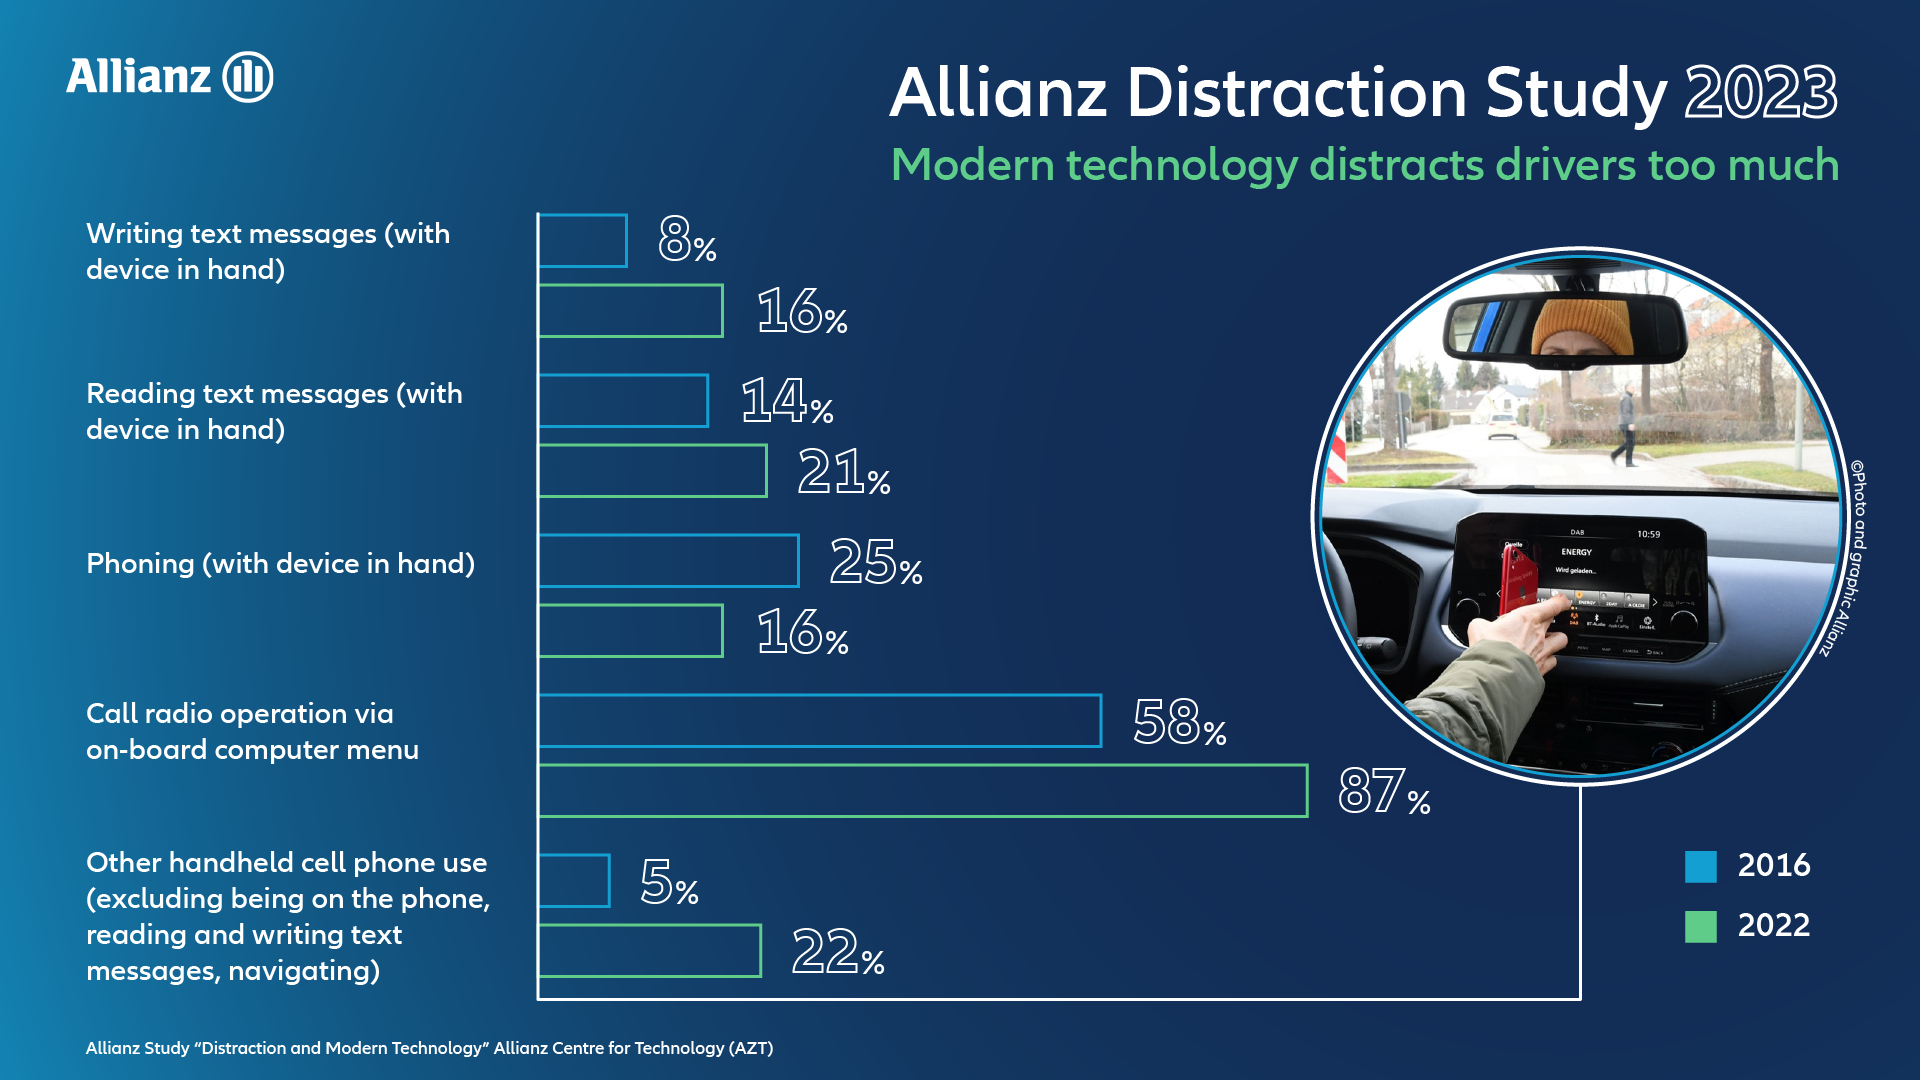
\includegraphics[width=0.8\textwidth]{Images_Thesis/Introduction_Related_Work/allianz-distraction-study-2023-technology-distracts-drivers.png}
\end{center}
\caption[Rise in distracted driving activities from 2016 to 2022]{Increase in instances of inattentive driving from 2016 to 2022. This figure illustrates the upward trend in various activities, such as reading text messages on a mobile phone while driving, from 2016 to 2022. These activities have played a role in the rise of distracted driving behavior. Source:~\citep{study_new_Allianz2023}}
\label{fig:allaianz_dd_2023}
\end{figure}

\section{Motivation}
Driver distraction stands as a significant cause of road accidents, necessitating rigorous research to foster a safer environment for road users~\citep{bing_li_2022new, in_vehicle_cameras_9618784, M1_regan2011driver, M2_young2007driver, moslemi2021computer}.~Such research aligns with the United Nations' 2030 goal to decrease road traffic fatalities and injuries substantially.~Traditionally, in computer vision, driver distraction detection has leveraged supervised learning algorithms, which depend on labeled data. However, acquiring this data is often expensive and labor-intensive.~Furthermore, supervised learning may not sufficiently generalize across diverse driving conditions, underscoring the need for unsupervised or self-supervised learning methods ~\citep{bing_li_2022new}.~Recent technological advances have equipped vehicles with various sensors and cameras, significantly enhancing the capability to monitor a broad spectrum of driver actions~\citet{in_vehicle_cameras_9618784, martin2019drive_and_act_2019_iccv}.~The \gls{daa} Dataset~\citep{martin2019drive_and_act_2019_iccv} presents a precious resource for pushing the boundaries of current research in driver activity recognition and distraction detection.~This dataset includes multiple data modalities, multi-view images, hierarchical labeling, and a detailed differentiation between various driver actions~\citep{martin2019drive_and_act_2019_iccv}.~These attributes combined establish it as an exceptional platform for extensive research and analysis. 

The primary objective of this research is to conduct a comprehensive exploration of the \gls{daa} Dataset~\citep{martin2019drive_and_act_2019_iccv} aimed at enhancing our understanding and detection of driver distractions.~This study engages in meticulous experimentation and analysis to assess the efficacy of using \gls{rgb} (color) and \gls{inr} (Gray Scale) imaging modalities from the \gls{daa} video dataset~\citep{martin2019drive_and_act_2019_iccv}.~A focal point of this research is extracting and creating image datasets and addressing dataset imbalances.

In advancing the field of driver distraction detection, this thesis utilizes advanced pre-trained vision transformer encoders.~It explores their application across different image modalities and views, testing their adaptability and generalizability.~The comparative analysis includes an encoder trained using a supervised learning technique and the one developed through \gls{ssl} framework DINOv2~\citep{dinov2_oquab2023dinov2}.~The sole purpose of this analysis is to highlight the performance of encoders trained using different techniques like supervised and \gls{ssl} on driver distraction detection and to evaluate the impact of various data modalities and image views on the accuracy and generalization of distraction detection.

Ultimately, this thesis aims to enhance driving safety, aligning with global safety objectives significantly.

\section{Research Questions}
\label{section:research_questions}
This thesis embarks on an exploration guided by these essential research questions:
\begin{itemize}
    \item \textbf{Practical Challenges:}~How can the issue of data imbalance in the \gls{daa} dataset~\citep{martin2019drive_and_act_2019_iccv} be addressed?~Is it possible to employ unsupervised learning techniques for this purpose, and if so, how can they be effectively implemented?
    
    \item \textbf{Effectiveness of \gls{ssl} Models:}~What are the benefits and drawbacks of using vision transformer encoders pretrained using \gls{ssl} based approaches, such as \gls{dino}~\citep{dinov2_oquab2023dinov2} over supervised learning based encoder, for detecting driver distraction?
    
    \item \textbf{Generalization Capabilities:}~How do different image views, such as the right top view and the front top view in the \gls{daa} dataset~\citep{martin2019drive_and_act_2019_iccv}, impact the detection of driver detection using computer vision?~Additionally, does a vision transformer~\citep{Vit_Paper_Dosovitskiy2020AnII} encoder pre-trained using a self-supervised learning approach maintain consistent performance on driver distraction detection tasks or generalize well across different views at hand?
    
    \item \textbf{Data Modality Impact:}~What are the impacts of varying data modalities, such as \gls{rgb} and \gls{inr} images, on detecting driver distractions? Furthermore, does the vision transformer encoder pre-trained using the self-supervised learning approach DINOv2~\citep{dinov2_oquab2023dinov2} demonstrate effective generalization across these modalities?
\end{itemize}

\section{Brief Outline of the Thesis}
The structure of the rest of the thesis is as follows:
\begin{itemize}
    \item \textbf{Chapter 2: Related Work} - A thorough literature review examines existing methods and technologies relevant to driver distraction detection.~This chapter highlights the limitations of conventional supervised learning approaches and highlights the necessity for innovative unsupervised or self-supervised learning models.~It also highlights the practical challenges with \gls{daa} dataset and identifies the research gaps this thesis aims to address.
    
    \item \textbf{Chapter 3: Background} - This chapter details the essential methodologies employed in this thesis.~It explains the working principle of the HDBSCAN~\citep{HDBSCAN_algo_campello2013density} clustering algorithm and vision transformer~\cite{Vit_Paper_Dosovitskiy2020AnII} and introduces relevant mathematical functions and terminology necessary for subsequent discussions.~Furthermore, it explains the self-supervised learning-based framework DINO~\citep{dino_caron2021emerging}, as well as the DINOv2 framework~\citep{dinov2_oquab2023dinov2}.
    
    \item \textbf{Chapter 4: Proposed Methods} - This chapter provides a comprehensive explanation of the innovative dataloader implementation, as well as a methodology to compare it with the traditional dataloader. This chapter also provides descriptions of the methodologies used in supervised learning-based encoder experiments and self-supervised learning-based encoder experiments.~Furthermore, this chapter discusses the theoretical foundations of the selected methods and explains their relevance in addressing the research goals outlined in the section~\ref{section:research_questions}.
    
    \item \textbf{Chapter 5: Experiments and Results} - This section delves into the experimental setup, highlighting the datasets utilized and the hyperparameter choices made. It also presents the implementation and results of the previously outlined methodologies across all experiments, offering a comprehensive analysis of the findings. Moreover, it specifically addresses the research questions posed in section~\ref{section:research_questions}.
    
    \item \textbf{Chapter 6: Conclusions and Future Work} - Concluding the thesis, this section integrates the findings, and identifies potential areas for future research to foster continued advancements in the field.
\end{itemize}

%% Please note that we have introduced automatic line number generation
%% into the style file for \LaTeXe. This is to help reviewers
%% refer to specific lines of the paper when they make their comments. Please do
%% NOT refer to these line numbers in your paper as they will be removed from the
%% style file for the final version of accepted papers.

%\begin{center}
%   \url{http://www.iclr.cc/}
%\end{center}
% The formatting instructions contained in these style files are summarized in
% sections \ref{gen_inst}, \ref{headings}, and \ref{others} below.